\newpage
\chapter{Реализация}\label{ch:chapter_2}

\section{Установка инструментария}

На текущей стадии разработки приложения отладка происходит в специальной среде
Scratchbox.

Scratchbox "--- набор инструментов для кросс-компиляции, предназначенный для
разработки приложений для встраиваемых Linux-систем. Scratchbox представляет
собой <<песочницу>>, в которой все действия разработчика изолированы от реальной
Linux-системы, на которой она запущена.

Внутри <<песочницы>> своя файловая система со своим домашним каталогом и другими
системными каталогами. Домашний каталог терминального сервера доступен из
Scratchbox по пути /host\_home/имя\_пользователя/. Таким образом, все примеры,
задания и прочие необходимые файлы могут размещаться и редактироваться в
домашнем каталоге терминального сервера, а сборка и запуск приложения могут
осуществляться в <<песочнице>> без перемещения файлов.

Установка гостевой ОС:
\begin{enumerate}
\item
Установка Scratchbox
\item
Устанавка Xephyr X11 - программное обеспечение, необходимое для запуска Maemo SDK. Оно обеспечивает экран устройства для разработчика. Имея права суперпользователя (root), выполняем команду \textbf{sudo apt-get install xserver-xephyr}.
\item
Установка Maemo SDK.\\
Для продолжения установки необходимо добавить текущего пользователя в группу sbox:\\
\textbf{newgrp sbox}\\
Далее нужно загрузить скрипт:\\
\textbf{
wget http://repository.maemo.org/stable/5.0/maemo-sdk-\textbackslash\\ install\_5.0.sh\\
chmod a+x ./maemo-sdk-install\_5.0.sh\\
./maemo-sdk-install\_5.0.sh}\\
Заходим в Scratchbox и выполняем все действия в нем:\\
\textbf{/scratchbox/login}\\
Если получено сообщение об отсутствии прав, нужно добавить пользователя следующей командой:\\
\textbf{sudo /scratchbox/sbin/sbox\_adduser USERNAME yes}
\item
Установка приложений Nokia\\
\textbf{sb-conf select FREMANTLE\_X86}
Для начала необходимо получить адрес источника обновлений и добавить их в список источников. Адрес можно узнать, перейдя по ссылке: \textit{http://tablets-dev.nokia.com/eula/index.php}\\
\textbf{echo "deb http://repository.maemo.org/ fremantle/<md5 хеш>\textbackslash\\
nokia-binaries" \textgreater\textgreater /etc/apt/sources.list}\\
Затем нужно обновить и установить следующие пакеты:\\
\textbf{apt-get update
fakeroot apt-get install nokia-binaries}\\
При возникновении проблем на этом этапе, рекомендуется повторить команду с параметром *--fix-missing*:
\textbf{fakeroot apt-get install nokia-binaries --fix-missing}
\item
Установка библиотеки Qt.\\
Для возможности сборки проектов с использованием библиотеки Qt, необходимо установить дополнительные пакеты, зайдя предварительно в оболочку:\\
\textbf{/scratchbox/login\\
fakeroot apt-get install libqt4-gui libqt4-dev}
\item
Сборка и запуск Qt-приложений
Предварительно нужно запустить эмулятор устройства, на котором будет выполняться приложение.
Выйдя из оболочки Scratchbox, нужно запустить Xephyr в новом окне:\\
\textbf{/scratchbox/logout\\
Xephyr :2 -host-cursor -screen 800x480x16 -dpi 96 -ac -kb \&}\\
В другом окне консоли заходим в Scratchbox, нужно указать окно для эмулятора и запустить его:\\
\textbf{/scratchbox/login\\
export DISPLAY=:2\\
af-sb-init.sh start}\\
Директория с файлами проекта должна быть доступна из окружения Scratchbox. Заходим в нее:\\
\textbf{cd ~/myQTProjectDir}\\
Создаем файл проекта, make-файлы и собираем проект:\\
\textbf{qmake -project\\
qmake\\
make}\\
Запуск приложения:\\
\textbf{run-standalone.sh ./myQTApp}
\end{enumerate}

\section{Реализация графического отображения диаграммы}

Первым этапом реализации задачи по отображению модели диаграммы является проектировании архитектуры взаимодействия классов модели и классов вида.
При проектировании архитектуры были учтены такие факторы, как работа с очень большим количеством графических элементов "--- узлов диаграммы и поддержка прокрутки для больших диаграмм. Диаграмму с взаимодействием классов сцены и классов модели можно видеть в приложении~\ref{ap:uml_scene} на рис.~\ref{ris:uml_scene}

Классами для отображения диаграммы были выбраны QGraphicsItem и
QGraphicsScene, т.к. они специально оптимизированы для отображения большого числа графических элементов. Классы NodeDelegate и MindMapDelegate являются посредниками между классами вида и классами модели: данные классы рассчитывают положение узлов на сцене.

Модель диаграммы связей не содержит информацию о расположении узлов в пространстве, поэтому необходима реализация алгоритма расчета координат каждого узла на сцене, на уровне классов посредников.

Основная идея алгоритма в том, чтобы уделить внимание только высоте элемента. Она должна быть достаточной, чтобы поместить текст и оформление узла.

\subsection{Расчет высоты элемента}

Основная секция алгоритма "--- это расчет высоты узла. Высота узла должна быть равна высоте поддерева этого узла. Если узел не содержит потомков, то его высота состоит из высоты текста и высоты оформления узла. Рис.~\ref{ris:node_single} показывает расчет высоты отдельного узла.
\begin{figure}[h!]
\centering
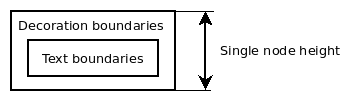
\includegraphics[width=0.5\linewidth]{node-single}
\caption{Расчет высоты узла}
\label{ris:node_single}
\end{figure}

Рис.~\ref{ris:node_complex}  описывает расчет высоты узла, если он имеет дочерние узлы. Если сумма высот дочерних узлов больше чем высота родительского узла, то данная сумма должна быть объявлена как высота данного узла. В противном случает должна использоваться высота данного узла.

\begin{figure}[h!]
\centering
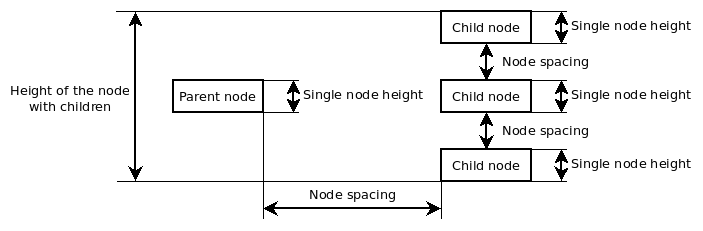
\includegraphics[width=\linewidth]{node-complex}
\caption{Расчет высоты узла с учетом высоты поддерева}
\label{ris:node_complex}
\end{figure}

Алгоритм расчета высоты узла:
\begin{lstlisting}
class MindMapDelegate{
	...
	def nodeHeight(self):
		...
	def height(self):
		sum = 0
		for childNode in self.__childs:
			sum += childNode.nodeHeight()
		if nodeHeight() < sum:
			return sum
		return nodeHeight()
	...
}
\end{lstlisting}

В примере метод nodeHeight() рассчитывает высоту самого узла. А метод height() рассчитывает высоту узла с учетом высоты дочерних узлов.

\subsection{Расчет положения узлов}

Для позиционирования узлов на сцене, необходимо определить базовую точку. Базовую точку можно видеть на рис.~\ref{ris:node_calculation}. Мы принимаем в расчет что узел может корректно отрисовать себя относительно базовой точки.

Позиция узла "--- это позиция в родительских координатах, то есть позиция базовой точки текущего узла идентируется из базовой точки родительского узла по осям $X$ и $Y$.

Все вычисления выполняются с использованием нижних элементов.
\begin{figure}[h!]
\centering
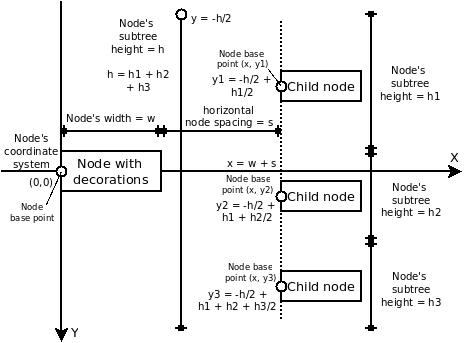
\includegraphics[width=0.8\linewidth]{node-calculation}
\caption{Расчет координат узла}
\label{ris:node_calculation}
\end{figure}

Горизонтальное смещение "--- это небольшой промежуток между всеми дочерними узлами и родительским узлом
$X$ равен сумме ширины родительского узла и величины горизонтального промежутка между узлами $X = w + s$.

Вертикальное смещение немного сложнее. Положим, что базовая точка узла "--- это половина высоты узла и родительский узел уже находится на середине высоты. Позиции дочерних узлов рассчитываются относительно базовой точки родительского, то есть относительно координаты $(0, 0)$.

Размещение узлов должно производиться относительно высоты родительского поддерева, а не относительно высоты родительского узла. Это учитывается потому что высота узла может превышать высоту поддерева.

Шаги, необходимые для вычисления позиции дочерних узлов:
\begin{enumerate}
\item
Рассчитать высоту родительского поддерева $(h = h1+h2+h3)$
\item
Найти верхнюю точку первого дочернего узла $(y=-h/2)$
\item
Рассчитать смещение по $y$ базовой точки узла $(y1=y+h1/2)$
\item
Установить позицию для дочернего узла $(x, y1)$
\item
Обновить верхнюю точку для следующего дочернего узла\\ $(y=y+h1)$
\item
Перейти на шаг 3, сдвинув соответственно значения\\ $(y1 \to y2, h1 \to h2)$
\end{enumerate}

Так же на сцене располагаются кнопки для управления масшабом карты. Результат работы можно видеть в приложении~\ref{ap:screenshot} на рис.~\ref{ris:main_view}

\section{Реализация контекстного меню узла}\label{sec:context_menu}

Задача контекстного меню "--- вызов наиболее востребованных операций над выбранным узлом диаграммы: сворачивание/разворачивание узла, добавление новых дочерних узлов и удаление выбранного узла, редактирование текста и выбор пиктограмм для узла.

Удобство работы с меню является одним из определяющих факторов простоты и скорости выполнения редактирования диаграммы.
Библиотека Qt поддерживает стандартное контекстное меню в виде списка названий операций, но в нашем случае оно будет выглядеть очень громоздко, поэтому было решено сделать анимированное меню в виде круглых кнопок, располагающихся по дуге. Ввиду особенностей мобильного устройства были выбраны достаточно большие размеры кнопок, чтобы обеспечить удобное управление пальцами, не используя стилус.

В качестве реализации анимации был взят Animation Framework библиотеки Qt. Он содержит все необходимые инструменты для реализации качественной анимации с минимальными затратами.

\subsection*{Алгоритм анимации меню}

\subsubsection*{Выбор радиусов эллипса}

При расчете размеров эллипса нужно учитывать размер кнопок меню. В данном случае размер кнопок равен 64x64 пикселя, так как граница эллипса должна проходить через центр кнопок. Так же нужно учесть небольшой запас, чтобы кнопки не соприкасались друг с другом. В итоге получим следующий алгоритм:
\begin{lstlisting}
rect = self._getItemViewRect()
self.__basePoint = rect.center()
if rect.width() > 100:
	self.__radiusOne = rect.width() / 2.0 + 32
else:
       self.__radiusOne = 82
if rect.height() > 60:
	self.__radiusTwo = rect.height() / 2.0 + 32
else:
	self.__radiusTwo = 62 
\end{lstlisting}
где rect "--- прямоугольник узла, \_\_basePoint "--- центр прямоугольника.
\begin{figure}[h!]
\centering
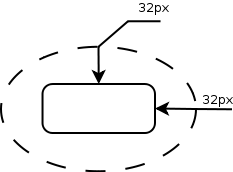
\includegraphics[width=0.3\linewidth]{menu/ellipse}
\end{figure}

\subsubsection*{Вычисление координат кнопок}
Для вычисления координат кнопок меню на границе эллипса нужно знать угол, относительно оси X. 
Для расположения кнопок по эллипсу зададимся шагом угла и минимальным расстоянием между кнопками.
Пусть начальные координаты первой кнопки меню задаются углов равным $1.2\pi$ радиана.
Тогда следующие координаты будут вычисляться по следующему алгоритму:
\begin{lstlisting}
angle = startAngle
angleStep = math.pi / 60
for each button:
	curPos = self._calculatePosition(angle)
	button.setPos(curPos)
	while True:
		angle += angleStep
		nextPos = self._calculatePosition(angle)
		if distance(curPos, nextPos) >=MIN_DISTANCE:
			if not self._isButtonInside(*nextPos):
				return
			break
\end{lstlisting}

Результат можно видеть в приложении~\ref{ap:screenshot} на рис.~\ref{ris:context_menu}.

\section{Реализация редактора текста узла}\label{sec:node_text_editor}

Библиотека Qt не имеет стандартного диалога для редактирования текста, поэтому возник вопрос о создании эргономичного редактора текста для приложения.
При разработке редактора текста нужно учитывать малые размеры экрана, поэтому было решено оставить в главном окне редактора только основные кнопки форматирования текста.

Большую часть экрана занимает поле для набора текста, оно может работать в нескольких режимах: редактирование простого текста и редактирование форматированного текста (в формате HTML).

Выбор семейства и размер шрифта осуществляется в отдельном окне, так как это довольно редкая операция и ее можно ее можно убрать из основного окна редактора.

Данный редактор работает в двух режимах: редактирование простого текста и редактирование HTML. В режиме HTML возможно редактирование как текста, так и исходного кода страницы. 

Режимы работы редактора показаны на рис.~\ref{ris:text_editor} в приложении~\ref{ap:screenshot}.

\section{Реализация поддержки пиктограмм в узлах}\label{sec:node_icons_support}

Использование пиктограмм в узлах повышает информативность диаграммы. С их помощью можно информировать пользователя о приоритете той или иной подзадачи или текущем статусе.
Для поддержки пиктограмм возникают такие задачи как загрузка пиктограмм в программу и диалог выбора некоторого списка пиктограмм из большой таблицы для конкретного узла.
Пиктограммы хранятся в отдельной папке, программа загружает те из них, которые указаны в настройках. Это дает большую гибкость настройки для конечного пользователя "--- возможность использования пользовательских пиктограмм.
Диалоговое окно для выбора пиктограмм разделено на две части: в верхней части находится таблица загруженных пиктограмм, а в нижней "--- список выбранных пиктограмм для узла. Выбор пиктограммы в таблице осуществляется простым кликом по ней, после чего она добавляется в конец списка.
При клике на пиктограмму в списке, она удаляется. Так же пиктограммы можно перемещать по списку, для этого нужно выбрать пиктограмму и, не отпуская ее, переместить на нужное место. Окно выбора пиктограмм можно видеть на рис.~\ref{ris:icons_selector} в приложении~\ref{ap:screenshot}.